	%\documentclass[landscape,a0b,final,a4resizeable]{a0poster}
	%\documentclass[landscape,a0b,final]{a0poster}
	%\documentclass[portrait,a0b,final,a4resizeable]{a0poster}
	\documentclass[portrait,a0b,final]{a0poster}
	%%% Option "a4resizeable" makes it possible ot resize the
	%   poster by the command: psresize -pa4 poster.ps poster-a4.ps
	%   For final printing, please remove option "a4resizeable" !!
	
	\usepackage{amsmath}
	\usepackage{graphicx}
	\usepackage{epsfig}
	\usepackage{multicol}
	\usepackage{natbib}
	\usepackage{pstricks,pst-grad}
	\usepackage{subfigure}
	\usepackage{hyperref}
	\usepackage{csvsimple}
	
	%%%%%%%%%%%%%%%%%%%%%%%%%%%%%%%%%%%%%%%%%%%%%%%%%%%%
	%%%           document formatting parameters
	%%%%%%%%%%%%%%%%%%%%%%%%%%%%%%%%%%%%%%%%%%%%%%%%%%%%
	
	% DEFINE POSTER WIDTH
	\newenvironment{poster}{
	  \begin{center}
	  \begin{minipage}[c]{0.98\textwidth}
	}{
	  \end{minipage} 
	  \end{center}
	}
	% DEFINITION OF SOME METRICS
	\setlength{\columnsep}{3cm}
	\setlength{\columnseprule}{2mm}
	%\setlength{\parindent}{0.0cm}
	% DEFINITION OF FUNCTION TO SET POSTER BACKGROUND GRADIENT COLORS
	\newcommand{\backgroundcolor}[3]{
	  \newrgbcolor{cgradbegin}{#1}
	  \newrgbcolor{cgradend}{#2}
	  \psframe[fillstyle=gradient,gradend=cgradend,
	  gradbegin=cgradbegin,gradmidpoint=#3](0.,0.)(1.\textwidth,-1.\textheight)
	}
	% MAIN TITLE ENVIRONMENT
	\newenvironment{pcolumn}[1]{
	  \begin{minipage}{#1\textwidth}
	  \begin{center}
	}{
	  \end{center}
	  \end{minipage}
	}
	% SECTION TITLE DECORATION BOX (BLUE GRADIENT)
	\newrgbcolor{lcolor}{0. 0. 0.80}
	\newrgbcolor{gcolor1}{1. 1. 1.}
	\newrgbcolor{gcolor2}{.80 .80 1.}
	%
	\newcommand{\pbox}[4]{
	\psshadowbox[#3]{
	\begin{minipage}[t][#2][t]{#1}
	#4
	\end{minipage}
	}}
	
	% MY FIGURES
	% \myfig - replacement for \figure
	% necessary, since in multicol-environment 171231_training_matrix.eps
	% \figure won't work
	\newcommand{\myfig}[3][0]{
	\begin{center}
	  \vspace{0.5cm}
	  \includegraphics[width=#3\hsize,angle=#1]{#2}
	  \nobreak\medskip
	\end{center}}
	%
	% MY CAPTIONS
	% \mycaption - replacement for \caption
	% necessary, since in multicol-environment \figure and
	% therefore \caption won't work
	
	%\newcounter{figure}
	\setcounter{figure}{1}
	\newcommand{\mycaptionfig}[1]{
	  \vspace{0.25cm}
	  \begin{quote}%\centering
	    {{\bf Figure \arabic{figure}:} #1}
	  \end{quote}
	  \vspace{0.5cm}
	  \stepcounter{figure}
	}
	
	%\newcounter{table}
	\setcounter{table}{1}
	\newcommand{\mycaptiontab}[1]{
	  \vspace{0.25cm}
	  \begin{quote}%\centering
	    {{\bf Table \arabic{table}:} #1}
	  \end{quote}
	  \vspace{0.5cm}
	  \stepcounter{table}
	}
	
	% DEFINE FONT COMMANDS
	\newcommand{\fontbody}{\Large}
	%\newcommand{\fontbody}[1]{\textsf{#1}}
	\newcommand{\fonttitle}[1]{\veryHuge \textsf{#1}} 
	\newcommand{\fontheader}[1]{\Huge \textsf{#1}} 
	
	
	%%%%%%%%%%%%%%%%%%%%%%%%%%%%%%%%%%%%%%%%%%%%%%%%%%%%%%%%%%%%%%%%%%%%%%
	%%% Begin of Document
	%%%%%%%%%%%%%%%%%%%%%%%%%%%%%%%%%%%%%%%%%%%%%%%%%%%%%%%%%%%%%%%%%%%%%%
	
	\begin{document}
	
	% Set document size
	\large
	
	\backgroundcolor{1. 1. 1.}{1. 1. 1.}{0.5}
	
	\vspace*{0.5cm}
	
	
	\newrgbcolor{lightblue}{0. 0. 0.80}
	\newrgbcolor{white}{1. 1. 1.}
	\newrgbcolor{whiteblue}{.80 .80 1.}
	
	
	\begin{poster}
	
	%%%%%%%%%%%%%%%%%%%%%
	%%% Header
	%%%%%%%%%%%%%%%%%%%%%
	
	\begin{center}
	%\begin{pcolumn}{1}
	\pbox{0.98\textwidth}{}{linewidth=2mm,framearc=0.3,linecolor=lightblue,fillstyle=gradient,gradangle=0,gradbegin=white,gradend=whiteblue,gradmidpoint=1.0,framesep=0.25em}{
	\begin{minipage}[c][10cm][c]{0.1\textwidth}
	  \begin{center}
	    \includegraphics[width=12cm,angle=0]{img_tmp/tagc_logo.eps}
	    \includegraphics[width=12cm,angle=0]{img_tmp/inserm.eps}
	  \end{center}
	\end{minipage}
	\begin{minipage}[c][9cm][c]{0.7\textwidth}
	  \begin{center}
	%Microarray analysis of chicken and mouse presomitic mesoderm along the posterior-anterior axisS
	%    {\sc \Huge Microarray analysis of chicken and mouse}\\[4.mm]
	%    {\sc \Huge presomitic mesoderm along the posterior-anterior axis}\\[2.mm]
	%\vspace{1cm}
	    { \fonttitle{Analysis of gene regulatory properties} }\\[4.mm]
	    { \fonttitle{underlying trait pleiotropy} }\\[2.mm]
	    \huge Aitor Gonz\'alez$^*$\\[2.mm]
	    \large TAGC Laboratory, Aix-Marseille Univ, INSERM UMR1090, 13288 Marseille, France\\[2.mm]
	    \large $^*$Email: aitor.gonzalez@univ-amu.fr
	  \end{center}
	  \end{minipage}
	\begin{minipage}[c][10cm][c]{0.1\textwidth}
	    \includegraphics[width=12cm,angle=0]{img_tmp/DIRCOM-Logo-FSS.eps}
	  \begin{center}
	  \end{center}
	\end{minipage}
	} % end pbox
	%\end{pcolumn}
	\end{center}
	
	%%%%%%%%%%%%%%%%%%%%%
	%%% Content
	%%%%%%%%%%%%%%%%%%%%%
	
	\vspace{0.5cm} % intersection space
	
	%%% Begin of Multicols-Enviroment
	\begin{multicols}{2}
	
	%%%%%%%%%%%%%%%%%%%%%
	%%% Background
	
	\begin{center}\pbox{0.8\columnwidth}{}{linewidth=2mm,framearc=0.1,linecolor=lightblue,fillstyle=gradient,gradangle=0,gradbegin=white,gradend=whiteblue,gradmidpoint=1.0,framesep=0.5em}{\huge \begin{center}\fontheader{Background and Objectives}\end{center}}\end{center}
	
	\section*{Background} 
	
	\begin{enumerate}
	\item Genome-wide association studies (GWAS) map genotypes to traits.
	\item Here we use this GWAS database: The IEU OpenGWAS project\\ \url{https://gwas.mrcieu.ac.uk}
	\item The large number of available GWAS have allowed to define pleiotropic regions in the genome \citep{2019.Posthuma.Watanabe}.
	\item Most GWAS loci are non-coding but the gene regulatory basis of pleiotropy is not well understood.
	\item Expression quantitative trait loci (eQTL) map genotypes to expression phenotypes.
	\item Here we use this eQTL database: The EBI eQTL Catalogue\\ \url{https://www.ebi.ac.uk/eqtl}
	\item Databases of GWAS and eQTL studies allow large colocalization analysis \citep{2021.Li.Mu}.
	\item The R package coloc performs colocalization tests between genetic traits:\\ \url{https://CRAN.R-project.org/package=coloc}
	\end{enumerate}
	
	\section*{Objectives} 
	
	\begin{enumerate}
	\item To develop an eQTL/GWAS variant colocalization pipeline
	\item To investigate gene regulatory properties underlying trait pleiotropy
	\end{enumerate}
	
	\vspace{0.5cm} % intersection space
	
	%%%%%%%%%%%%%%%%%%%%%
	%%% Results
	
	\begin{center}\pbox{0.8\columnwidth}{}{linewidth=2mm,framearc=0.1,linecolor=lightblue,fillstyle=gradient,gradangle=0,gradbegin=white,gradend=whiteblue,gradmidpoint=1.0,framesep=0.5em}{\begin{center}\fontheader{Results}\end{center}}\end{center}
	
	%%%%%%%%%%%%%%%%%%%%%%%%%%%%%%%%%%%%%%%%%%%%%%%%%%%%%%%%%%%%%%%%%%%%%%%%%%%%%%%%
	% FIGURE 1 web interface
	\begin{minipage}{\columnwidth}
	    \begin{center}
		    \begin{minipage}{1\columnwidth} 
			    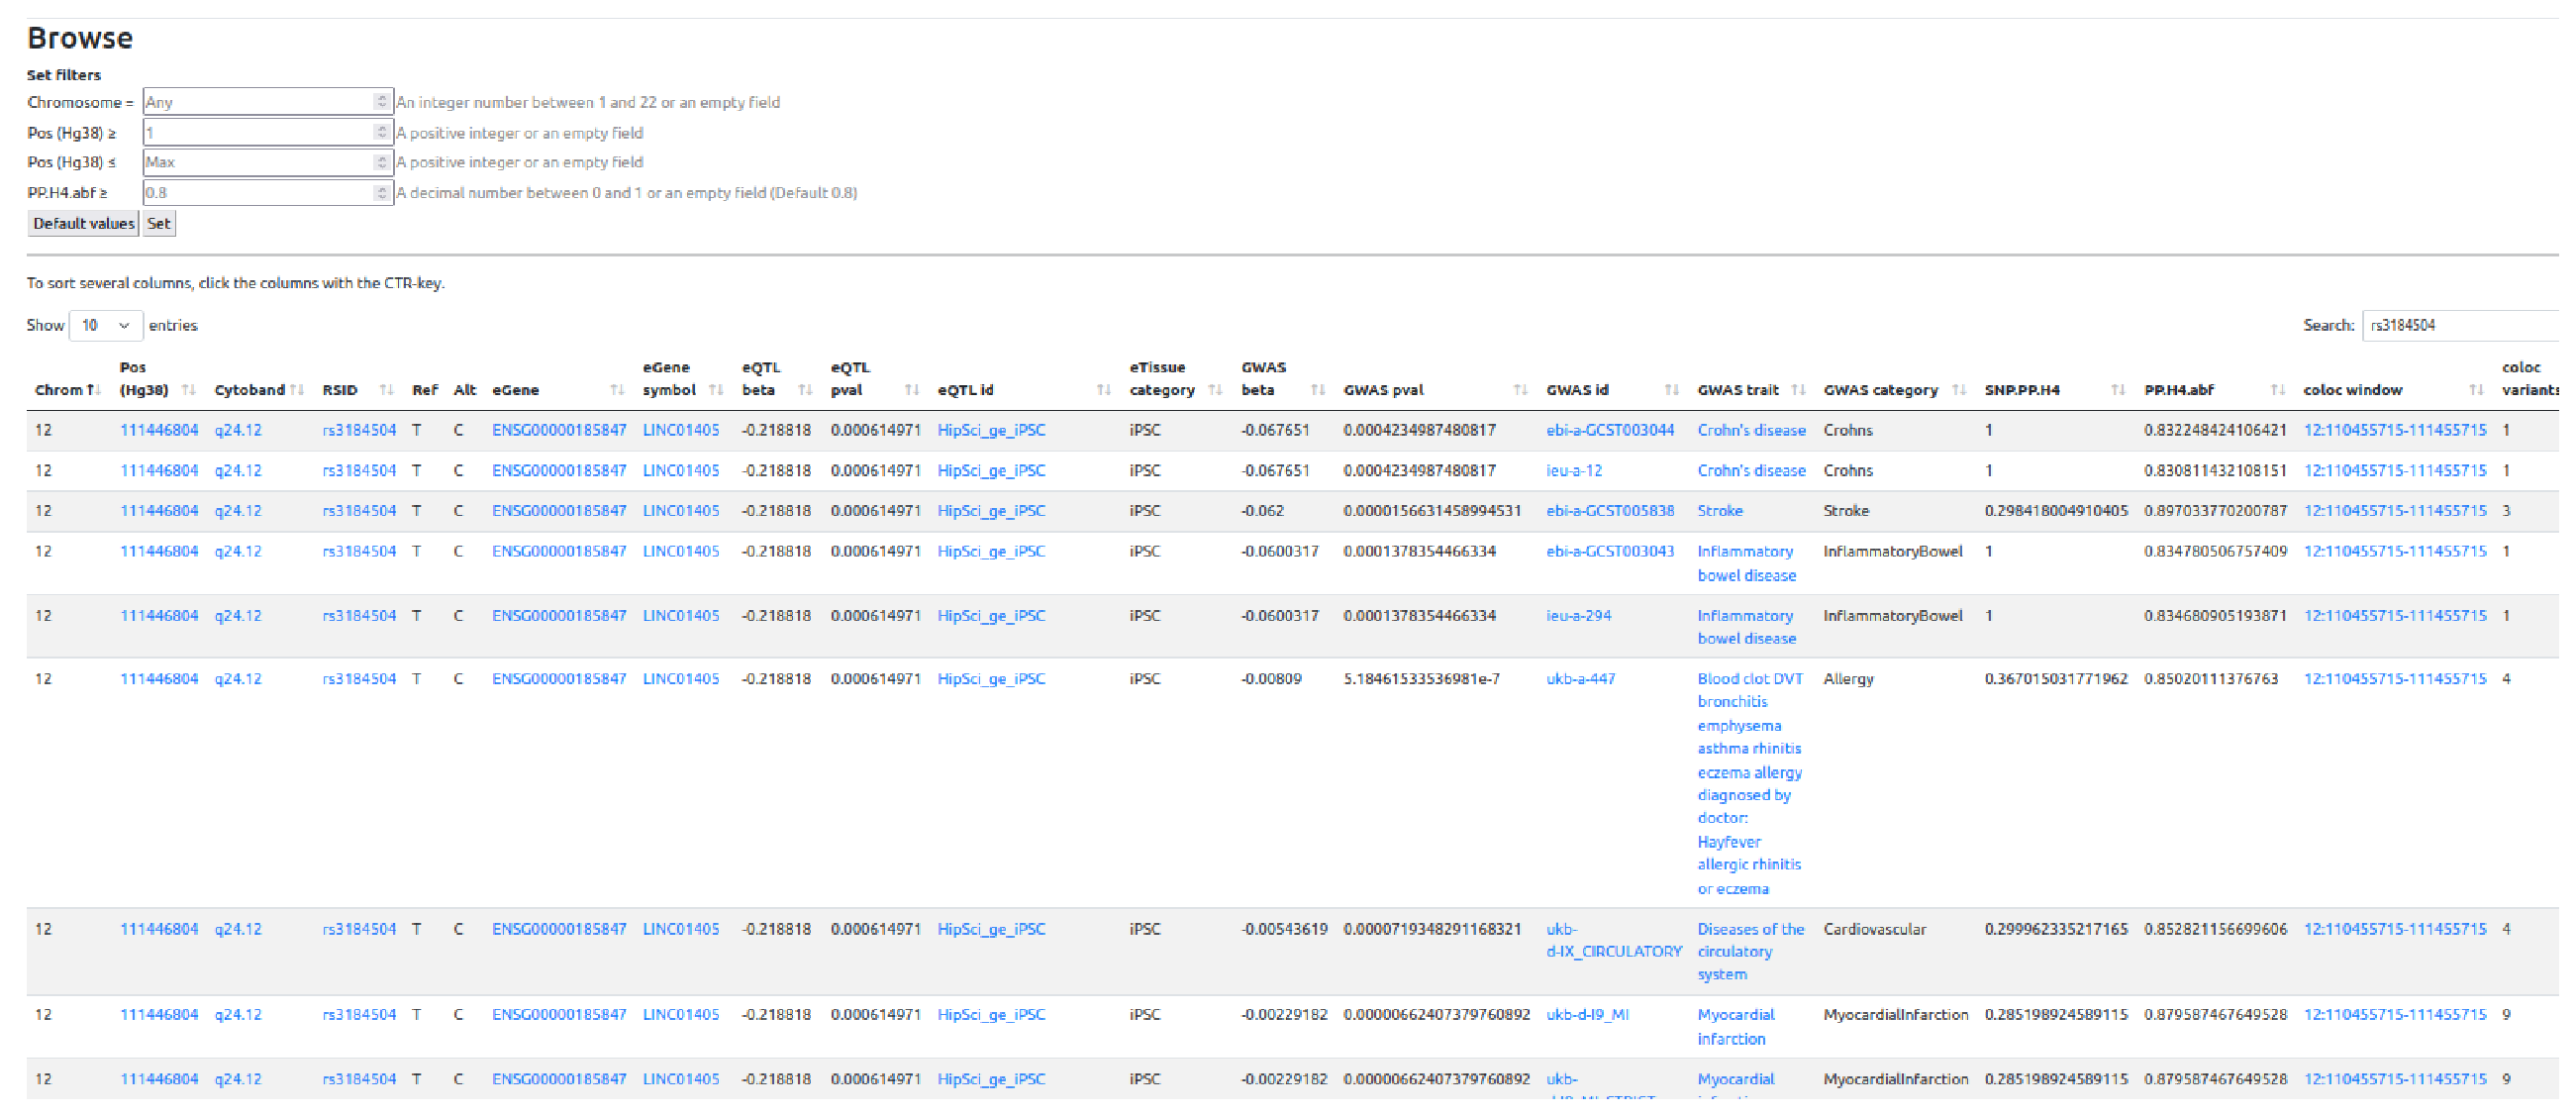
\includegraphics[width=\columnwidth]{img/web.eps}
		    \end{minipage}
		    \mycaptionfig{Web interface with the results of the colocalization pipeline for the most pleiotropic variant rs3184504.}
	    \end{center}
	\end{minipage}
	
	\vspace{0.5cm} % intersection space	
	
	%%%%%%%%%%%%%%%%%%%%%%%%%%%%%%%%%%%%%%%%%%%%%%%%%%%%%%%%%%%%%%%%%%%%%%%%%%%%%%%%
	%
	% Tab 1: Winner variants
	%
	%%%%%%%%%%%%%%%%%%%%%%%%%%%%%%%%%%%%%%%%%%%%%%%%%%%%%%%%%%%%%%%%%%%%%%%%%%%%%%%%
	
	% full size table is table*
	\begin{minipage}{\columnwidth}
	   \begin{center}
	\scriptsize
	\csvreader[separator=tab,
	tabular=ccrrp{0.4\textwidth},
	head,
	table head=\bfseries Chrom. & \bfseries Cytoband & \bfseries Pos (hg38) & \bfseries Variant & \bfseries GWAS Categories\\\hline,
	]{../ms/fig/tab_rsid_most_pleiotropic.tsv}{}% use head of csv as column names
	{\csvcoli\ & \csvcolii\ & \csvcoliii\ & \csvcoliv & \csvcolvi}% specify your coloumns here
	\large  % normal size
		    \mycaptiontab{Pleiotropic regions involving 5 or more GWAS categories. Genomic coordinates are given for the hg38 assembly.}
	    \end{center}
	\end{minipage}
	
	\vspace{0.5cm} % intersection space	
	
	%%%%%%%%%%%%%%%%%%%%%%%%%%%%%%%%%%%%%%%%%%%%%%%%%%%%%%%%%%%%%%%%%%%%%%%%%%%%%%%%
	% FIGURE 2 downstream regulation
	\begin{minipage}{1\columnwidth}
	    \begin{center}
		    \begin{minipage}{\columnwidth} 
\includegraphics[width=\textwidth]{img_tmp/david_pleio_3.eps}
\includegraphics[width=\textwidth]{img_tmp/david_pleio_2.eps}
		    \end{minipage}
		    \mycaptionfig{Gene ontology analysis of genes associated with eQTLs (eGenes) of variants associated to three (\textbf{Upper}) and two (\textbf{Bottom}) GWAS categories compared to eGenes of variants associated to one GWAS category.}
	    \end{center}
	\end{minipage}
	
	\vspace{0.5cm} % intersection space
	
	%%%%%%%%%%%%%%%%%%%%%%%%%%%%%%%%%%%%%%%%%%%%%%%%%%%%%%%%%%%%%%%%%%%%%%%%%%%%%%%%
	% FIGURE 1 VEP
	\begin{minipage}{1\columnwidth}
	    \begin{center}
		    \begin{minipage}{0.32\columnwidth} 
			    \includegraphics[width=\columnwidth]{img_tmp/missense_variant.eps}
		    \end{minipage}
		    \begin{minipage}{0.32\columnwidth} 
			    \includegraphics[width=\columnwidth]{img_tmp/splice_region_variant.eps}
		    \end{minipage}
		    \begin{minipage}{0.32\columnwidth} 
			    \includegraphics[width=\columnwidth]{img_tmp/3_prime_UTR_variant.eps}
		    \end{minipage}
		    \mycaptionfig{Variant effect predictor (VEP) analysis as a function of the number of GWAS catategory number for three different consequences: Missense variant (\textbf{Left}), splice region variant (\textbf{Center}) and 3’ UTR variant (\textbf{Right})}
	    \end{center}
	\end{minipage}
	
	\vspace{0.9cm} % intersection space	
	
	%%%%%%%%%%%%%%%%%%%%%%%%%%%%%%%%%%%%%%%%%%%%%%%%%%%%%%%%%%%%%%%%%%%%%%%%%%%%%%%%
	% FIGURE 2 downstream regulation
	\begin{minipage}{1\columnwidth}
	    \begin{center}
		    \begin{minipage}{0.32\columnwidth} 
			    \includegraphics[width=\columnwidth]{img_tmp/pltbar_x_per_variant_etissue_y_egene.eps}
		    \end{minipage}
		    \begin{minipage}{0.32\columnwidth} 
			    \includegraphics[width=\columnwidth]{img_tmp/pltbar_x_per_variant_egene_y_etissue.eps}
		    \end{minipage}
		    \begin{minipage}{0.32\columnwidth} 
			    \includegraphics[width=\columnwidth]{img_tmp/pltbar_x_per_variant_egene_etissue_y_gwas.eps}
		    \end{minipage}
		    \mycaptionfig{Count of eGenes per variant-tissue (\textbf{Left}), samples of eQTLs (eTissues) per variant-eGene (\textbf{Center}) and GWAS categories per variant-eGene-eTissue (\textbf{Right}).}
	    \end{center}
	\end{minipage}
	
	\vspace{0.9cm} % intersection space
	
	%%%%%%%%%%%%%%%%%%%%%%%%%%%%%%%%%%%%%%%%%%%%%%%%%%%%%%%%%%%%%%%%%%%%%%%%%%%%%%%%
	% FIGURE 3 TFs
	\begin{minipage}{1\columnwidth}
	    \begin{center}
		    \begin{center}
			    \begin{minipage}{0.35\columnwidth} 
				    \includegraphics[width=\columnwidth]{img_tmp/bxplt_remaptf_per_rsid_flank_0.eps}
			    \end{minipage}
			    \begin{minipage}{0.6\columnwidth} 
			    \mycaptionfig{Binding count of transcription factors in the region surrounding pleiotropic variants (Radius 50 bp) as a function of the GWAS category count. }
			    \end{minipage}
		    \end{center}
	    \end{center}
	\end{minipage}
	
	\vspace{0.9cm} % intersection space
	
	%%%%%%%%%%%%%%%%%%%%%%%%%%%%%%%%%%%%%%%%%%%%%%%%%%%%%%%%%%%%%%%%%%%%%%%%%%%%%%%%
	% FIGURE 4 Model
	\begin{minipage}{1\columnwidth}
	    \begin{center}
		    \begin{minipage}{1\columnwidth} 
			    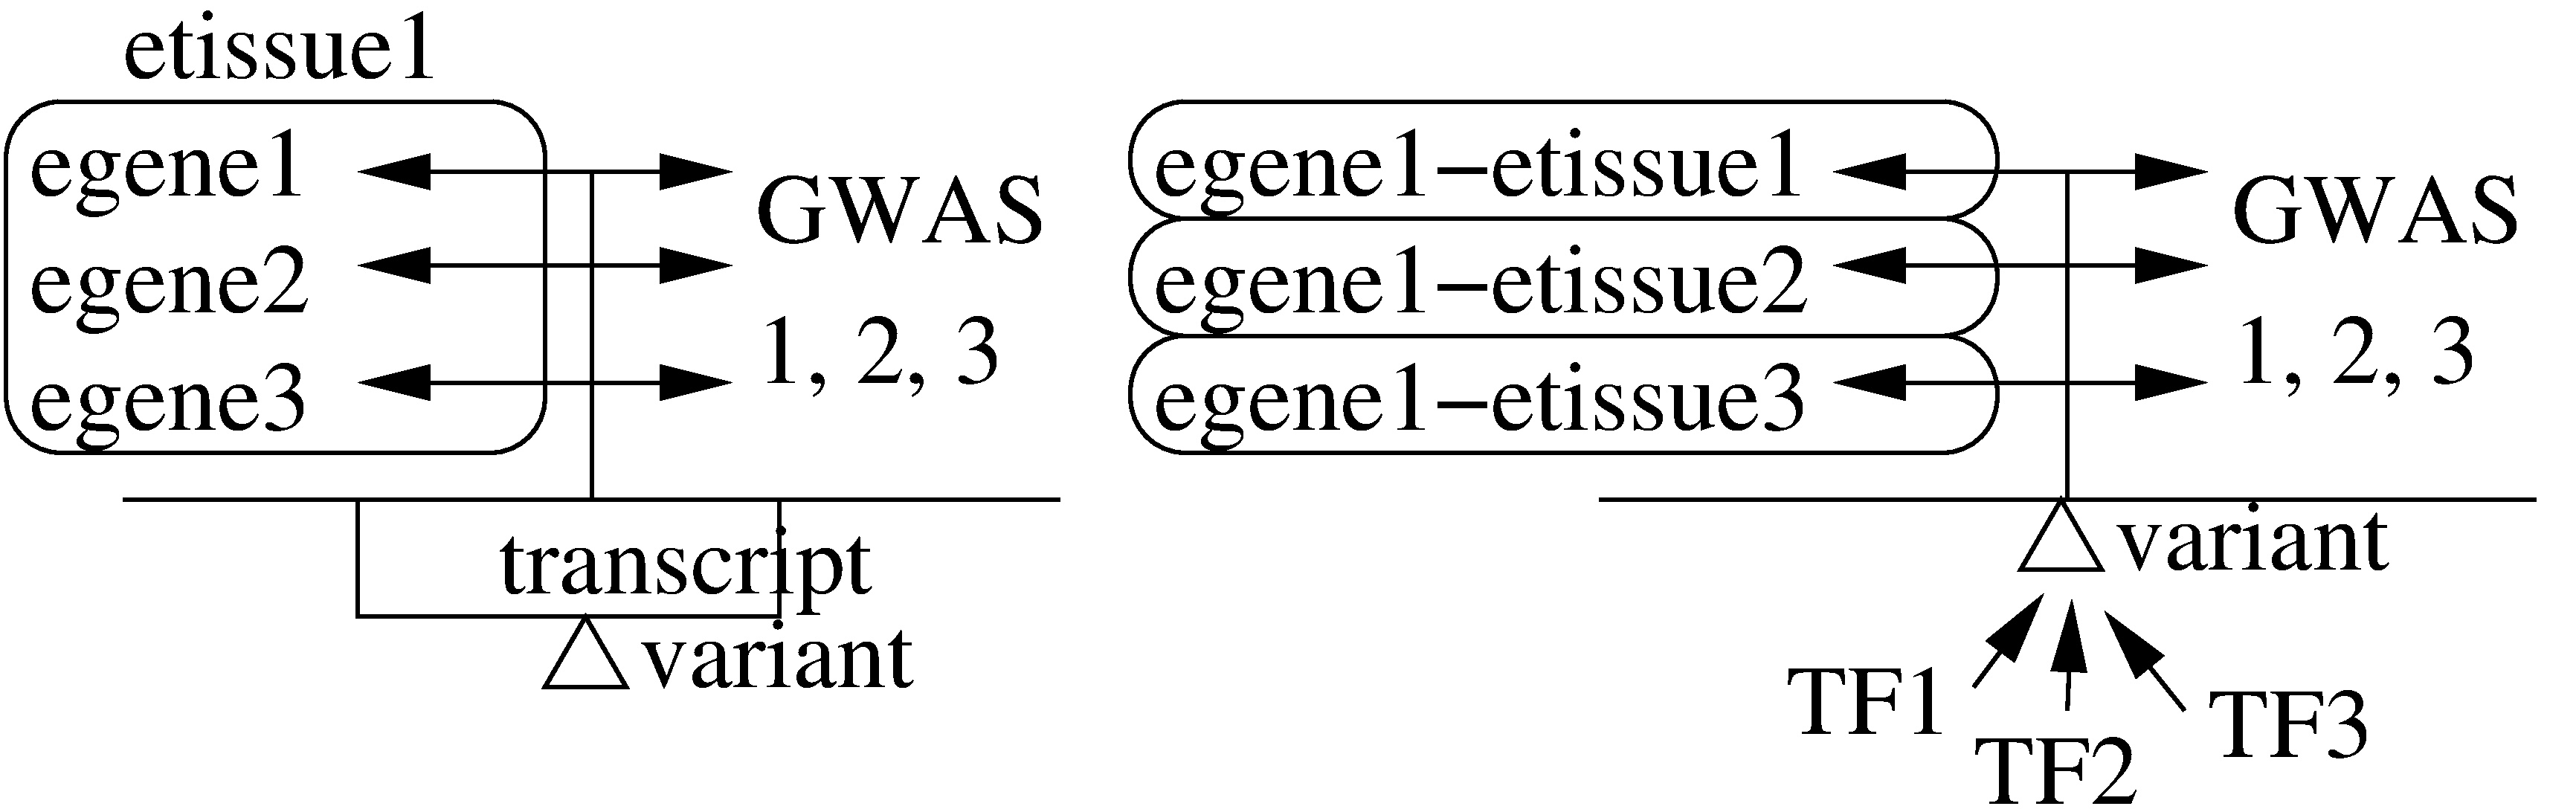
\includegraphics[width=\columnwidth]{img_tmp/graphical_summary.eps}
		    \end{minipage}
		    \mycaptionfig{Model of regulatory variant pleiotropy. I have investigated
	three possible mechanisms of pleiotropy. (\textbf{Left}), Pleiotropic variants have more
	eGenes that result in more functions and more phenotypes. This might arise
	from an enrichment of pleiotropic variants in splicing or 3’ UTR regions.
	(\textbf{Center}), I have also found that eGenes of pleiotropic variants are active
	in more etissues which result in more GWAS phenotypes. This might be
	explained from variants being bound by more transcription factors. (\textbf{Right}),
	Triplets of variant-eGene-eTissues are associated with more GWAS pheno-
	types, which directly affect the number of GWAS phenotypes. I have found
	that this might be explained by an enrichment of missense alleles.}
	    \end{center}
	\end{minipage}
	
	\vspace{0.9cm} % intersection space
	
	%%%%%%%%%%%%%%%%%%%%%
	%%% Conclusions and Future Directions
	
	\begin{center}\pbox{0.8\columnwidth}{}{linewidth=2mm,framearc=0.1,linecolor=lightblue,fillstyle=gradient,gradangle=0,gradbegin=white,gradend=whiteblue,gradmidpoint=1.0,framesep=0.5em}{\begin{center}\fontheader{Conclusions}\end{center}}\end{center}
	
	\begin{itemize}	
	\item We have developed a pipeline of eQTL/GWAS colocalization based on 127 eQTL studies and 150 GWAS (\textbf{Fig. 1}).
	\item These colocalization results are available in an easy to use web site (\textbf{Fig. 1}).
	\item We have computed a list of pleiotropic eQTLs (\textbf{Table 1}).
	\item eGenes of pleiotropic variants are enriched in immune related functions (\textbf{Fig. 2}).
	\item Pleiotropic variants are enriched in missense and splice region VEP effect consequences (\textbf{Fig. 3}).
	\item Pleiotropic eQTLs have more eGenes per variant-eTissue, are active in more eTissues per variant-eGene and are associated to more GWAS categories per variant-eGene-eTissue (\textbf{Fig. 4}).
	\item Pleiotropic variants bind more transcription factors (\textbf{Fig. 5}).
	\item We propose a model explaining the hypotheses underlying the pleiotropy for eQTLs (\textbf{Fig. 6}).
	\end{itemize}
	
	\normalsize
	\bibliographystyle{plain}
	\bibliography{../ms/ms_pleiotropy.bib}
	
	\end{multicols}
	
	
	\end{poster}
	
	\end{document}

